
Como dijimos anteriormente, el algoritmo tiene una complejidad de $\Theta(n + m)$. El algoritmo no tiene peor o mejor caso propiamente dichos (dado que es $\Theta(n + m)$ para todos los casos), pero veremos que, tomando $n$ fijo y moviendo $m$, podemos hacer variar el tiempo que toma el algoritmo.



\begin{figure}[H]
 \centering
	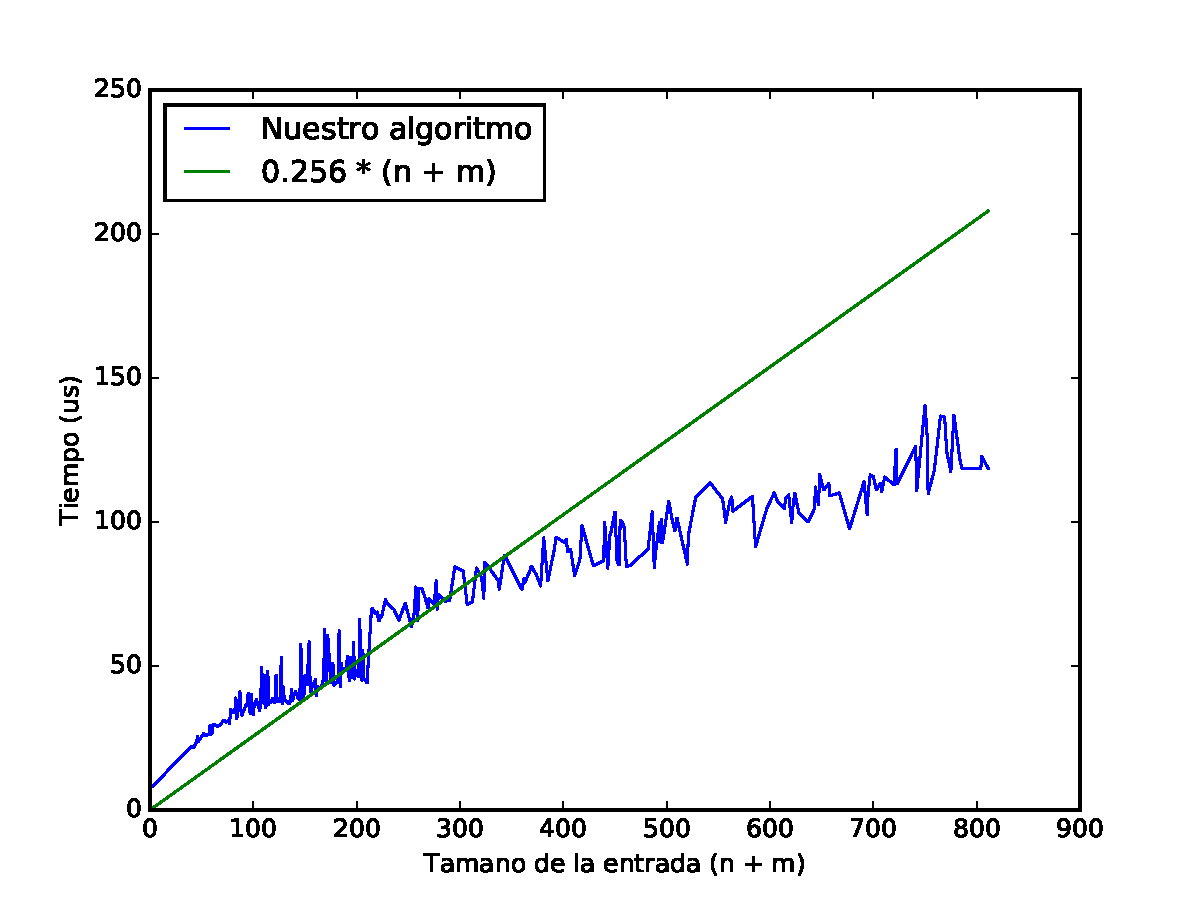
\includegraphics[width=0.9\textwidth]{img/exp/problema1-promedio.pdf}
	\caption{\footnotesize Tiempo que toma el algoritmo en $\mu$s para una entrada de tamaño $n + m$. $m$ al azar entre $n-1$ y $\frac{n(n-1)}{2}$.}
	\label{fig:problema1-promedio}
\end{figure}

Como se observa, la implementación tiene complejidad lineal sobre $n + m$, como era esperado.

Para confirmarlo, usamos el gráfico de la funcion $\frac{T(n + m)}{n + m}$, donde $T$ es el tiempo que tarda el algoritmo para la entrada de tamaño dado.
Si vemos que converge a una constante, estaremos en el caso exacto de la definción de $\Theta(f(n))$.

\begin{figure}[H]
 \centering
	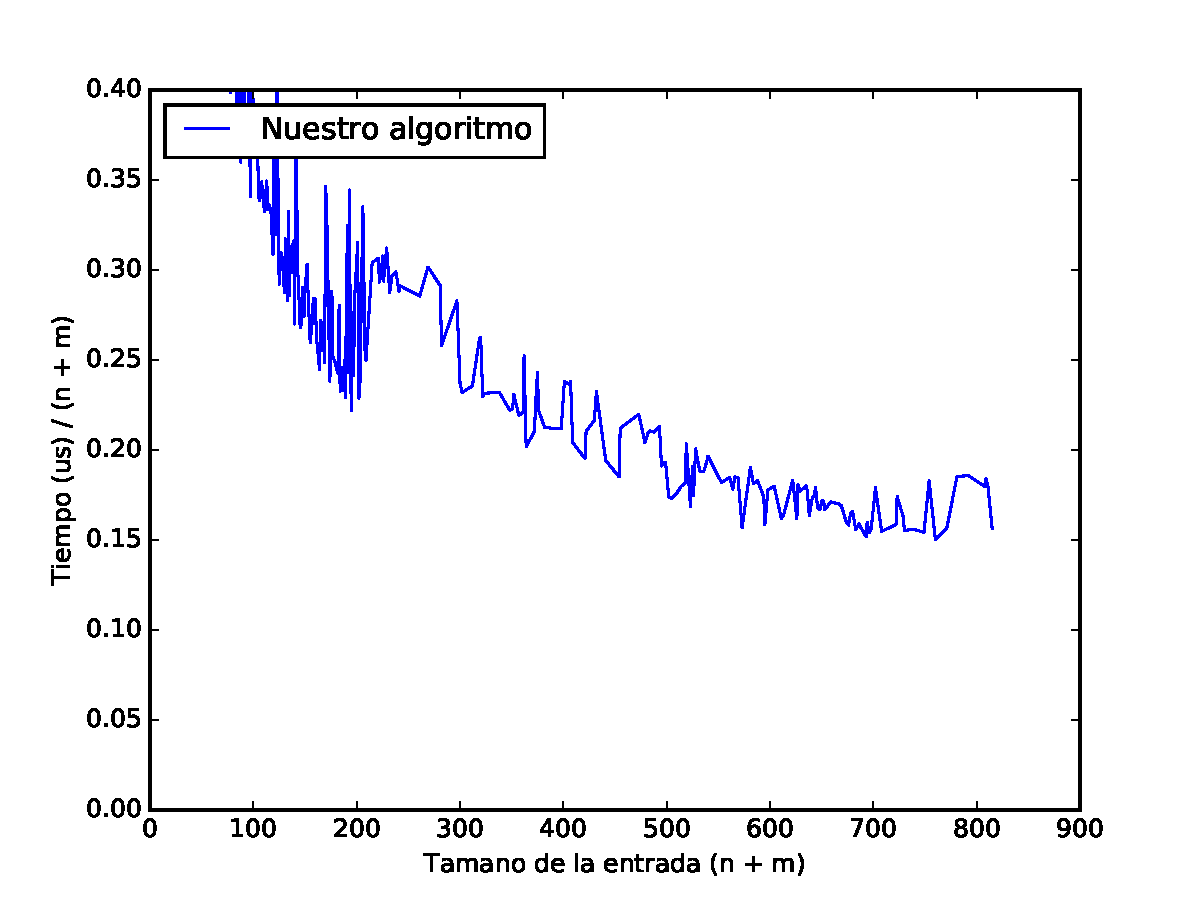
\includegraphics[width=0.9\textwidth]{img/exp/problema1-promedio2.pdf}
	\caption{\footnotesize Tiempo que toma el algoritmo en $\mu$s dividido $n + m$ para una entrada de tamaño $n + m$.  $m$ al azar entre $n-1$ y $\frac{n(n-1)}{2}$}
	\label{fig:problema1-promedio2}
\end{figure}

El ruido del gráfico se debe a que la escala es otra y distorciona las distancias entre los puntos. Sin embargo, se puede observar que converge a una constante, como era esperado.


Como habiamos dicho anteriormente, aunque el algoritmo es $\Theta(n + m)$, podemos ver casos particulares del algoritmo, en el que $n$ está fijo y movemos $m$ y ver como se comporta el algoritmo.

Primero veamos el caso en el que $m \in O(n)$. Esperaríamos que el algoritmo aquí tenga una complejidad de $O(n + m) = O(n + n) = O(n)$. Esto fue confirmado experimentalmente, como se muestra a continuación.

\begin{figure}[H]
 \centering
	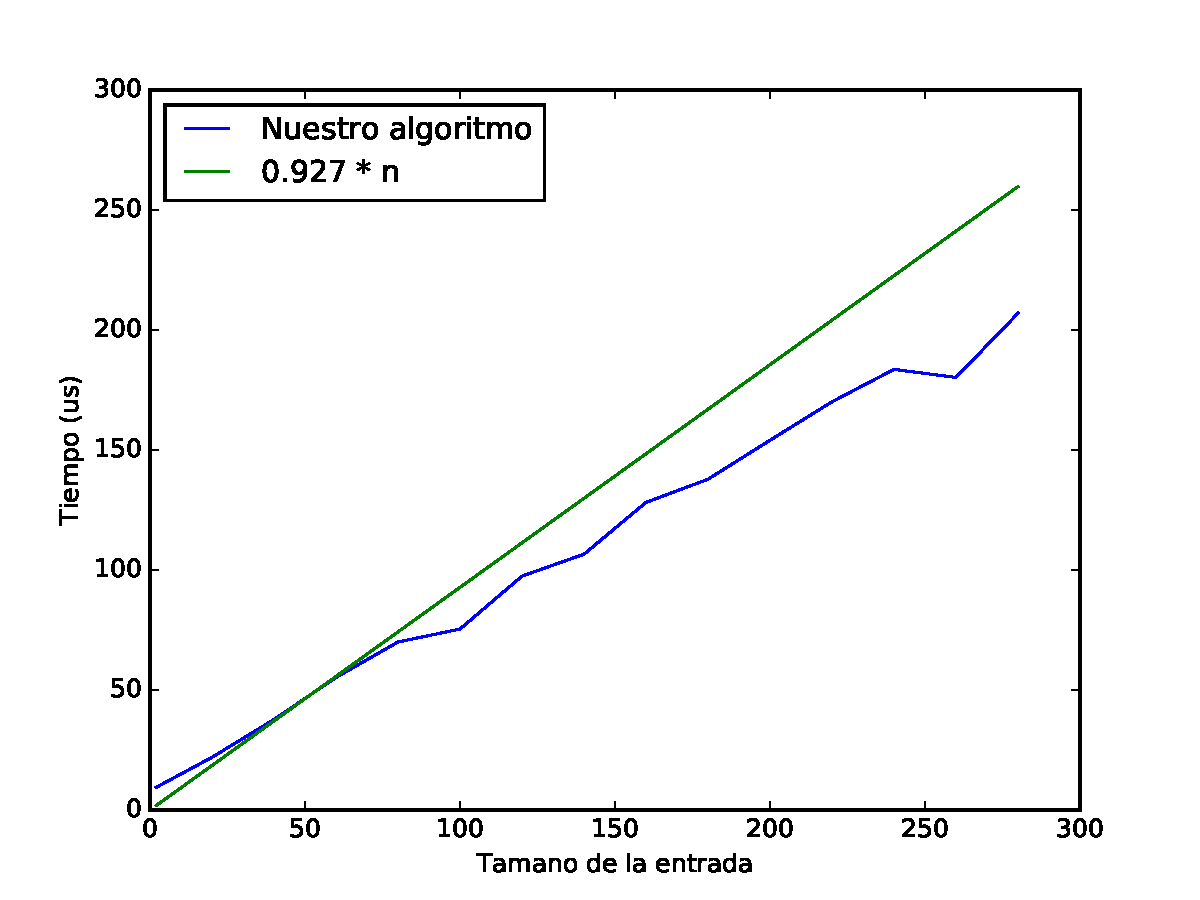
\includegraphics[width=0.9\textwidth]{img/exp/problema1-mejor.pdf}
	\caption{\footnotesize Tiempo que toma el algoritmo en $\mu$s para una entrada de tamaño $n$ ($m \in O(n))$.}
	\label{fig:problema1-mejor}
\end{figure}


Ahora veamos el caso en el que $m \in O(n^2)$. Esperaríamos que el algoritmo aquí tenga una complejidad de $O(n + m) = O(n + n^2) = O(n^2)$. Esto fue, nuevamente, confirmado experimentalmente.

\begin{figure}[H]
 \centering
	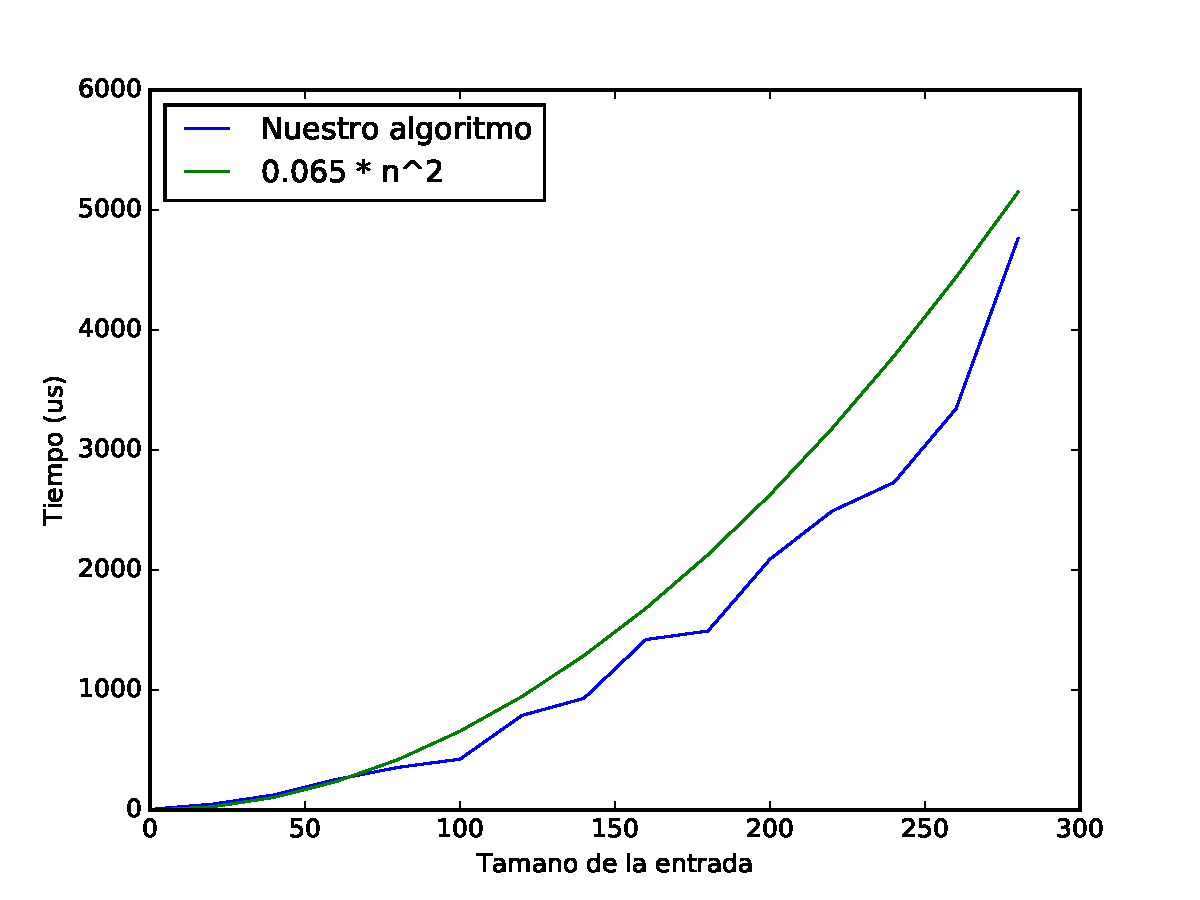
\includegraphics[width=0.9\textwidth]{img/exp/problema1-peor.pdf}
	\caption{\footnotesize Tiempo que toma el algoritmo en $\mu$s para una entrada de tamaño $n$ ($m \in O(n^2))$.}
	\label{fig:problema1-peor}
\end{figure}


Por último, como diremos en detalle en la siguiente sección, en la que explicamos la métodología de experimentación, en todos los experimentos anteriores asumimos que no importan la cantidad de caminos especiales de un grafo dado.

Esto es bastante obvio desde el punto de vista del algoritmo (pues es una consecuencia inmediata de que la complejidad esté dominada por la construcción del grafo), pero nos parece algo muy interesante verificarlo experimentalmente, dado que en este hecho se basan todos los experimentos anteriores.

Vale notar que, no obstante, sí puede haber pequeñas diferencias como consecuencia de que BFS ciertamente puede variar su performance a partir de cómo se conectan los vértices y cuántas aristas especiales hay. Pero esto afecta solo constantes, que se traducen en poco más que ruido en el gráfico.

Como puede verse en la siguiente figura, si tomamos $n$ y $m$ fijos, la cantidad de caminos especiales del grafo no afectan significativamente la performance del algoritmo.

\begin{figure}[H]
 \centering
	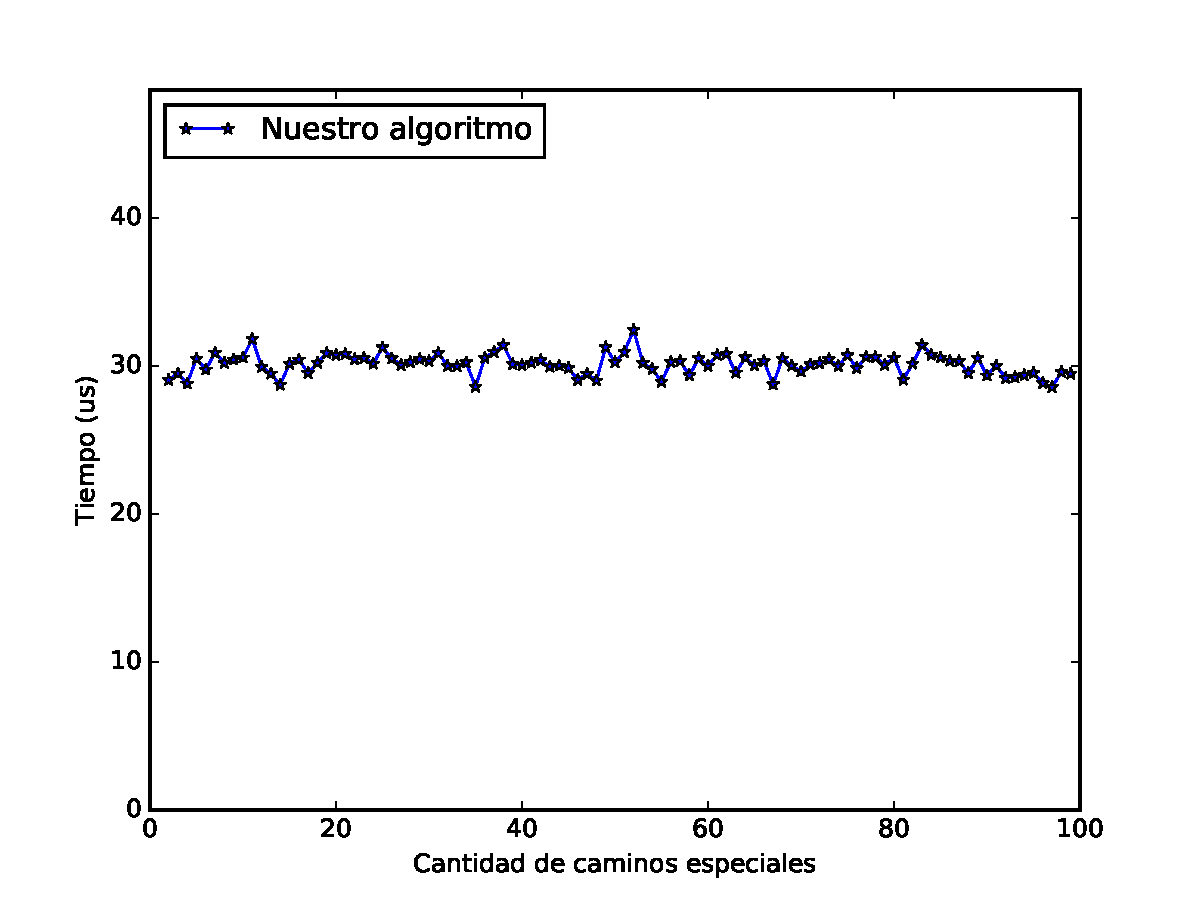
\includegraphics[width=0.9\textwidth]{img/exp/problema1-especiales.pdf}
	\caption{\footnotesize Tiempo que toma el algoritmo en $\mu$s para una entrada de tamaño $n = 15, m = 100$, variando la cantidad de caminos especiales.}
	\label{fig:problema1-especiales}
\end{figure}



\subsubsection{M\'etodo de experimentación}

Para la experimentación general del algoritmo, es decir, la verificación de que su complejidad era de $\Theta(n+m)$, generábamos distintos grafos al azar ($n$ al azar y $m$ elegido al azar tal que quede conexo).

En los casos particulares, dado $n$ fijo, tomamos $m = n - 1$ para el primer experimento y $m = \frac{n (n - 1)}{2}$ en el segundo.

Para la generación al azar de grafos utilizamos el algoritmo descripto en la sección \ref{subsec:grafos-aleatorios} del apéndice. Vale la pena aclarar cómo hicimos para decidir cuántas aristas especiales tendría el grafo. Primero, lo que hicimos fue notar experimentalmente que, con $n$ y $m$ fijos, si tomábamos distinta cantidad de caminos especiales (de 2 a $m$), la varianza de las mediciones era muy baja, es decir, la cantidad de caminos especiales de un grafo no afecta a la performance. 

Esto fue observado y comprobado experimentalmente. En consecuencia, para cada $n$ y $m$ fijo, tomamos grafos totalmente al azar, con cantidad de caminos especiales también al azar, y calculamos la mediana de todos los tiempos para determinar el tiempo total.
